\documentclass[a4paper,conference]{IEEEtran}
\usepackage{graphicx}
\usepackage{amsmath}
\usepackage{url}

\makeatletter
\newcommand{\authornewline}{
        \end{@IEEEauthorhalign}
        \hfill\mbox{}\par\mbox{}\hfill
        \begin{@IEEEauthorhalign}
}
\makeatother

\author{
    \IEEEauthorblockN{Hernán Alejandro Silva}
    \IEEEauthorblockA{
        Facultad Regional Avellaneda\\
        Universidad Tecnológica Nacional\\
        Buenos Aires, Argentina\\
        hernansilva2002@gmail.com
    }
    \and
    \IEEEauthorblockN{Elías Ramírez}
    \IEEEauthorblockA{
        Facultad Regional Avellaneda\\
        Universidad Tecnológica Nacional\\
        Buenos Aires, Argentina\\
        foo@gmail.com
    }
    \and
    \IEEEauthorblockN{Florencia Mincone}
    \IEEEauthorblockA{
        Facultad Regional Avellaneda\\
        Universidad Tecnológica Nacional\\
        Buenos Aires, Argentina\\
        foo@gmail.com
    }
    \authornewline
    \IEEEauthorblockN{Nicolás Lahorca}
    \IEEEauthorblockA{
        Facultad Regional Avellaneda\\
        Universidad Tecnológica Nacional\\
        Buenos Aires, Argentina\\
        foo@gmail.com
    }
    \and
    \IEEEauthorblockN{Luciano Justiniano}
    \IEEEauthorblockA{
        Facultad Regional Avellaneda\\
        Universidad Tecnológica Nacional\\
        Buenos Aires, Argentina\\
        foo@gmail.com
    }
}
\title{Detector de Partículas Beta}

\begin{document}
\maketitle
\begin{abstract}
    Constantemente los objetos que nos rodean emiten partículas que los sentidos
    humanos no son capaces de percibir. Estas partículas pueden ser
    perjudiciales para la salud y es necesario cuantificarlas y/o detectarlas
    para evitar o reducir la exposición a ellas. Para lograr ese objetivo, en
    este documento se presenta la realización de un dispositivo que cumpla la
    función de detectar un tipo de radiación, llamada radiación
    $\boldsymbol{\beta}$. En particular, se hará hincapié en la radiación por
    emisión de electrones, a este tipo de radiación se la conoce como radiación
    $\boldsymbol{\beta-}$. Además, se propone el análisis de su principio de
    funcionamiento, los materiales necesarios para su construcción y sus
    limitaciones.
\end{abstract}
\section{Introducción}
    El presente documento sirve como informe sobre el proyecto de fin de año de
    la asignatura Física Electrónica. Dicho proyecto se trata de un detector y
    contador de partículas beta, cubriendo de esta forma el tema de "Radiación"
    de la asignatura. Para más información sobre el proyecto, se recomienda
    visitar el repositorio del mismo que se encuentra en el siguiente enlace:
    (enlace al repo del proyecto).
\section{Principio de Funcionamiento}
    \subsection{¿Que son las radiaciones $\beta$?}
        Las radiaciones $\beta$ son un tipo de radiacion ionizante, la cúal se
        caracteriza por emitirse durante el proceso de desintegración o
        decaimento $\beta$. Dicho proceso puede producirse de dos diferentes
        formas.
        \begin{enumerate} 
            \item \textit{Emisión de electrones}: Un núcleo inestable de un
                átomo emite un electrón y un antineutrino, conviritiendo de esta
                manera un neutrón en un protón como \emph{Desintegración $\beta+$}.
            \item \textit{Emisión de positrones}: El núcleo inestable emite un
                positrón, es decir, un electrón cargado positivamente, junto con
                un neutrino. De esta forma se logra transformar un protón en un
                neutrón. Este proceso recibe el nombre de
                \emph{Desintegración $\beta+$}. 
        \end{enumerate}

        Generalmente, las fuentes más comunes de radiación de partículas $\beta$
        son piedras con pequeñas cantidades de uranio, y diferentes fuentes de
        potasio, como el cloruro de potasio (KCl), el cúal contiene baja
        cantidad del isótopo potasio 40 (K40), capáz de emitir partículas
        $\beta-$.

    \subsection{Formas de captar las partículas}
       El dispositivo electrónico más estudiado y utilizado para detectar
       la radiación de diferentes tipos de partículas es el diodo PIN o
       fotodiodo. Este es similar en cuanto a estructura a un diodo de juntura
       PN, la diferencia radica en que el PIN tiene una zona de material
       semiconductor intrínseco (zona I) entre la zona dopada positivamente (zona P) y la zona
       dopada negativamente (zona N).\par
       Al ser un material semiconductor, la zona I contiene átomos
       de silicio que, al momento de ser impactados por una partícula
       irradiada debido a una fuente radioactiva, genera la rotura de los
       enlaces covalentes del átomo, produciendo un \emph{par electrón-laguna}.
       La generación de este par tiene como consecuencia un pulso de corriente
       de decenas hasta cientos de microampere que atraviesan al diodo. Esta
       corriente puede ser medida. Además, cuando al diodo se lo polariza en
       forma inversa (cátodo con potencial más alto que el potencial del ánodo),
       se genera un campo eléctrico en la zona de
       \newpage
       \begin{figure}[!t]
           \centering
           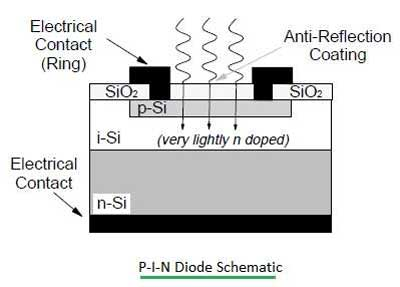
\includegraphics[width=2.5inch]{img/PIN_structure.jpg}
           \caption{Corte transversal de una estructura típica del diodo PIN}
           \label{fig:pin}
       \end{figure}

% Las malditas referencias. TODO: Sacar este comment.
\bibliographystyle{IEEEtran}
\bibliography{refs}
\nocite{*}
\end{document}
